\chapter{METODE PENENILITIAN}

\section{Garis Besar Penelitian}

Secara garis besar, penelitian ini akan melaksanakan pengembangan sistem monitoring mesin diesel berbasis \textit{IoT} yang akan diuji pada PT Bisma Jaya untuk meningkatkan efektivitas operasi dengan menekankan kecepatan minimum pada armada dan efisiensi biaya bahan bakar dengan memantau jumlah bahan bakar yang digunakan setiap harinya. Tampilan web akan dikembangkan menggunakan framework NextJS berbasis JavaScript dan sistem \textit{backend} menggunakan framework Django berbasis Python. Pengembangan sistem ini akan menggunakan metode Extreme Programming yang memiliki tahapan sebagai berikut: Exploration Phase, Planning Phase, Iteration to Release Phase, Productionizing Phase, Maintenance Phase, dan Death Phase.

\section{Diagram Alir Penelitian}

Metodologi pelaksanaan penelitian ini dapat dimodelkan menggunakan diagram alir sebagai berikut.

\begin{figure}[!h]
    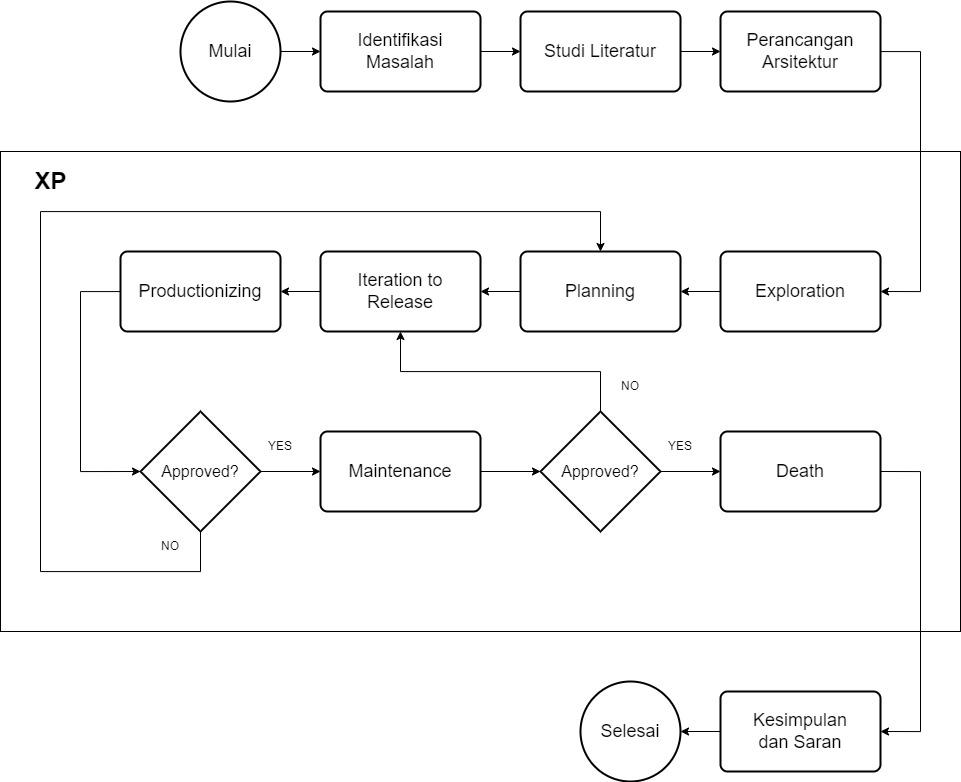
\includegraphics[width=1.1\linewidth, center]{images/metode/flowchart-penelitian.jpg}
    \caption{Diagram Alir Penelitian}
    \label{fig:flow-research}
\end{figure}


Pada Gambar 3.1 dapat dilihat bahwa penelitian ini diawali dengan melakukan identifikasi masalah dan studi literatur mengenai jurnal-jurnal dari penelitian relevan yang telah dilakukan sebelumnya. Kemudian, dilanjutkan dengan pengembangan sistem menggunakan metode \textit{Exteme Programming (XP)} yang terdiri dari Exploration Phase, Planning Phase, Iteration to Release Phase, Productionizing Phase, Maintenance Phase, dan Death Phase. Terakhir dilakukan pembuatan kesimpulan dan saran dari penelitian.

\section{Prosedur Penelitian}

Berikut penjelasan prosedur penelitian secara rinci berdasarkan tahapan-tahapan yang ditetapkan pada Gambar 3.1 sebagai pedoman penelitian ini.

\subsection{Identifikasi Masalah}

Penelitian ini dimulai dengan mengidentifikasi permasalahan yang ada di mitra. Ini dilakukan melalui dua cara, diskusi dengan seluruh \textit{stakeholder} yang terlibat dan observasi ke lapangan. Dari tahap ini akan dihasilkan rumusan masalah, tujuan, serta batasan-batasan penelitian.

\subsection{Studi Literatur}

Pada tahap ini dilakukan studi literatur dengan mengumpulkan berbagai referensi yang didapat dari jurnal, artikel ilmiah, dan sumber lainnya mengenai pengembangan sistem berbasis \textit{IoT}, teknologi-teknologi yang digunakan selama penelitian, dan perbandingan metodologi dalam pengembangan perangkat lunak.

\subsection{Pengembangan Sistem}

\subsubsection{Perancangan Arsitetur}

\begin{figure}[!h]
    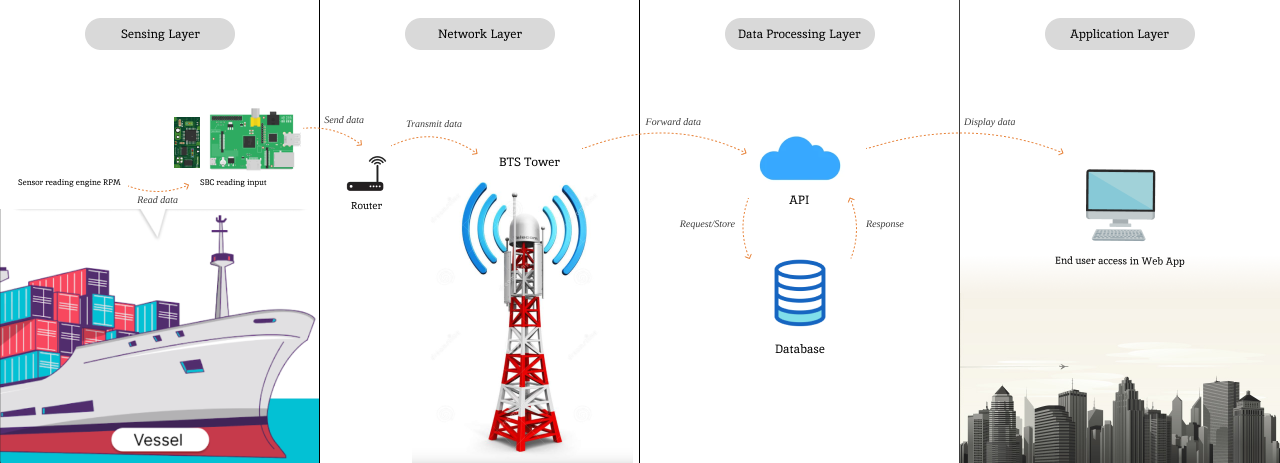
\includegraphics[width=1\linewidth, center]{images/metode/fig-system-archi.png}
    \caption{Arsitektur Sistem Monitoring bebasis IoT}
    \label{fig:system-archi}
\end{figure}

Gambar diatas merupakan arsitektur dari Sistem Monitoring berbasis IoT yang akan dikembangkan. Pertama, perangkat IoT akan dipasang di kapal untuk mengumpulkan data dari sensor. Data ini kemudian akan dikirim oleh router/modem LTE menuju server melalui API yang telah dibuat dan disimpan ke dalam basis data. Sebelum ditampilkan di aplikasi web, data ini akan diproses terlebih dahulu di \textit{Data Processing Layer} sehingga menghasilkan wawasan seperti data \textit{running hour} mesin, tren data kecepatan mesin, dan tren data konsumsi bahan bakar. Di layer terakhir, data akan ditampilkan dalam bentuk grafik untuk menganalisis tren data kecepatan dan konsumsi bahan bakar serta log data untuk mendapatkan informasi spesifik pada rentang waktu tertentu. Pada penelitian ini, difokuskan pada pengembangan untuk \textit{Network Layer}, \textit{Data Processing Layer}, dan \textit{App Layer} berdasarkan arsitektur IoT yang dibahas pada bab sebelumnnya.

\subsubsection{Extreme Programming}

\paragraph{\textit{Exploration Phase}}

    Kebutuhan yang dikumpulkan pada tahap identifikasi masalah kemudian dibuat dalam bentuk \textit{user story} untuk mendeskripsikan hasil yang diinginkan. Daftar \textit{user story} sementara dapat dilihat pada tabel berikut.

    \newpage

    \begin{longtable}[!h]
        {
            p{0.15\textwidth}
            p{0.15\textwidth}
            p{0.35\textwidth}
            p{0.35\textwidth}
        }
            \toprule
            \textit{Code} &
            \textit{Persona} &
            \textit{I want to} &
            \textit{So that can} \\ [0.5ex]
            \midrule

            US-01 &
            \textit{User} &
            \textit{Login} &
            Mengakses sistem sesuai dengan username dan password
            \\

            US-02 &
            \textit{User} &
            \textit{Logout} &
            Keluar dari sistem melalui tombol logout \\

            US-03 &
            \textit{User} &
            Melihat data historis kecepatan mesin &
            Memastikan armada bergerak dengan kecepatan mesin yang sesuai
            \\

            US-04 &
            \textit{User} &
            Melihat data historis konsumsi bahan bakar &
            Melakukan kontrol bahan bakar
            \\

            US-05 &
            \textit{User} &
            Melihat data historis \textit{running hour} &
            Memastikan operasi berjalan dengan optimal
            \\

            US-06 &
            \textit{User} &
            Melihat data log kecepatan per menit &
            Melihat detail kecepatan pada waktu spesifik
            \\

            US-07 &
            \textit{User} &
            Mencetak laporan kecepatan mesin harian &
            Mendapatkan laporan harian kecepatan mesin dengan format PDF
            \\

            US-08 &
            \textit{User} &
            Mencetak laporan harian konsumsi bahan bakar &
            Mendapatkan laporan harian konsumsi bahan baar dengan format PDF
            \\

            US-09 &
            \textit{User} &
            Mengunduh data log kecepatan mesin &
            Mendapatkan log kecepatan mesin dengan format CSV
            \\ [1ex]
            \bottomrule
        \caption{User Story Sementara}
        \label{tab:user-story}
    \end{longtable}

    Lebih lanjut, berdasarkan user story yang dibuat di tahap sebelumnya, akan dilakukan analisis dengan output perancangan user interface sistem dan skema basis data dalam bentuk entity relationship diagram (ERD) yang akan membantu dalam menggambarkan hubungan antar tabel. Berikut Entity Relationship Diagram sementara pada pengembangan Sistem Monitoring.


    \begin{figure}[!h]
        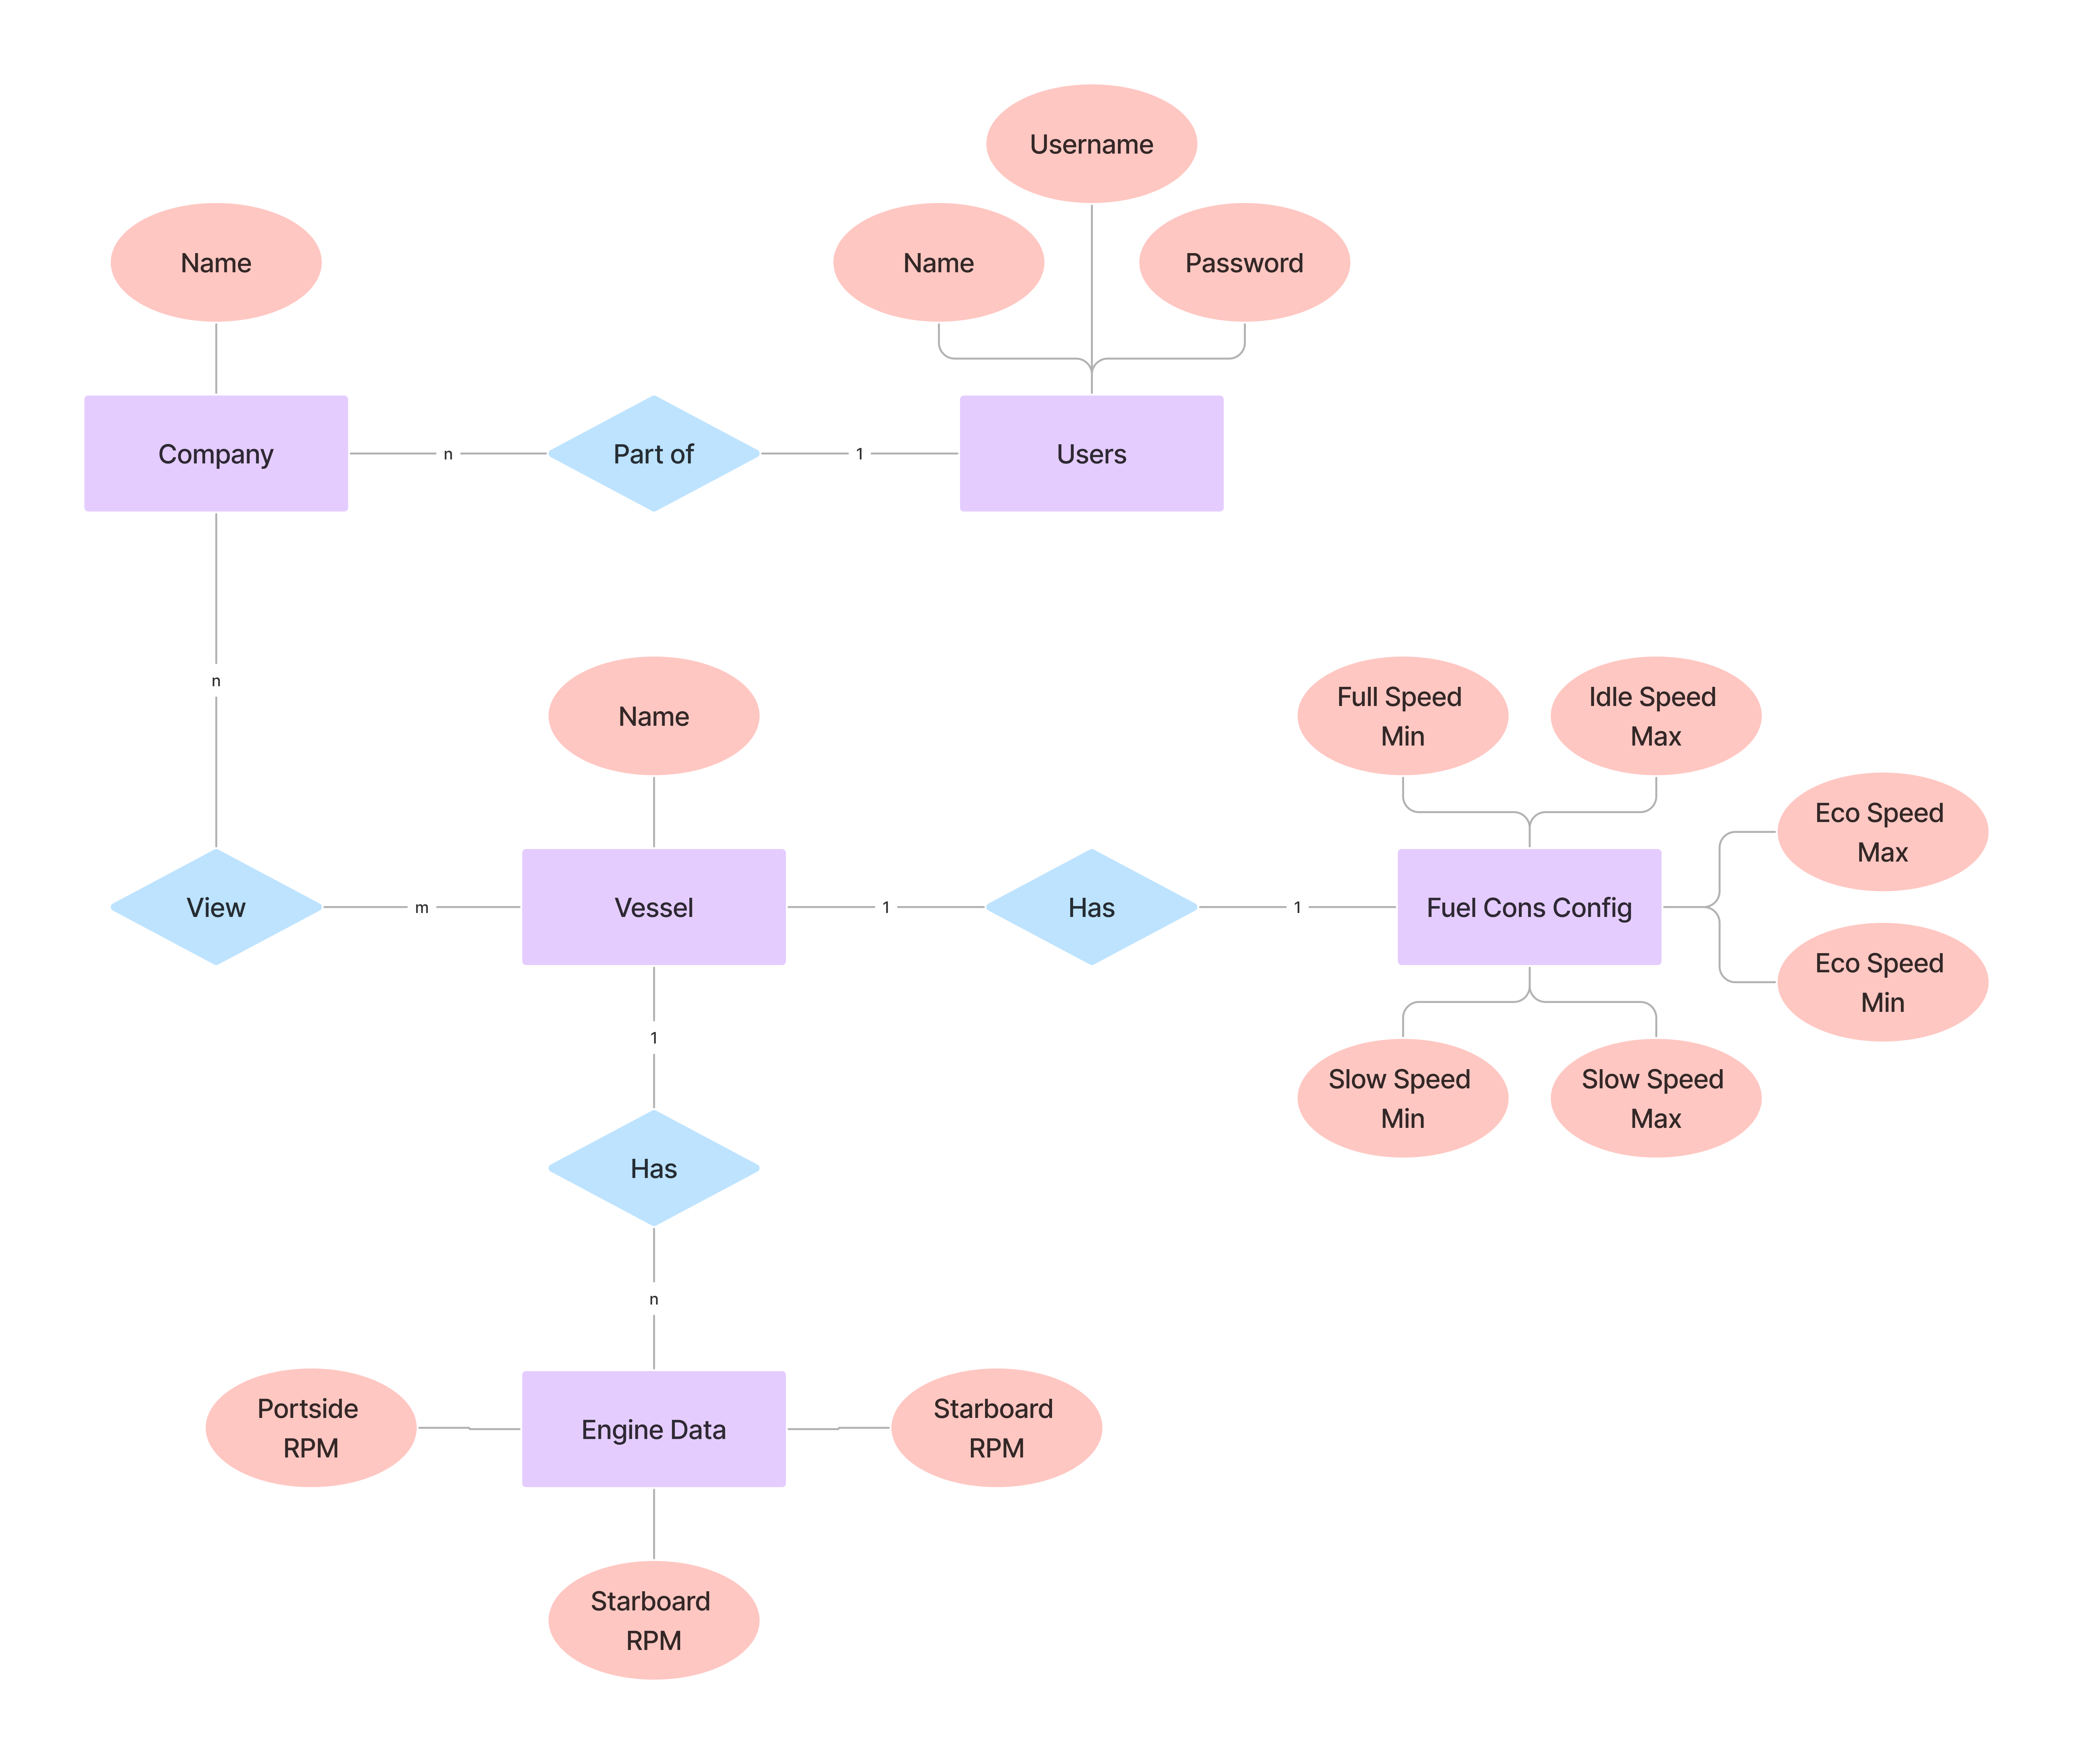
\includegraphics[width=1\linewidth, center]{images/metode/erd.png}
        \caption{Entity Relationship Diagram (ERD) Sementara}
        \label{fig:erd}
    \end{figure}

    \paragraph{\textit{Planning Phase}}

    User story yang dibuat pada tahap sebelumnya akan dikumpulkan dan disimpan berdasarkan prioritas. Tahap ini akan diulang kembali setelah melewati tahap testing sesuai dengan jumlah iterasi pengembangan.

    \paragraph{\textit{Iteration to Release Phase}}

    Fase ini terbagi menjadi beberapa bagian. Pertama, dilakukan analisis kebutuhan yang akan menghasilkan kebutuhan fungsional sistem dari task yang ditentukan; Kemudian, dilakukan desain wireframe sederhana untuk membantu pengembang dalam proses penyelesaian task dengan sesuai; Lalu, dilakukan tahap implementasi dari perancangan sistem. Dalam pengembangan dashboard digunakan framework NextJS untuk menghasilkan tampilan yang dinamis, kemudian digunakan framework Django yang berbasis bahasa Python untuk mengembangkan API agar perangkat IoT dapat mengirim data ke server. Setelah dilakukannya pengembangan seluruh task pada iterasi tersebut, setiap fungsi akan diuji melalui unit test sebelum akhirnya diunggah ke repositori dan akan diuji kembali setelahnya oleh mitra melalui metode black box testing. Jika terdapat umpan balik, maka tahapan akan diulang ke tahap desain untuk menyesuaikan permintaan mitra. Sebaliknya, jika mendapatkan persetujuan maka sistem akan masuk ke tahap berikutnya.

    \paragraph{\textit{Productionizing Phase}}

    Setelah melewati serangkaian \textit{whitebox testing} dan mendapatan persetujuan mitra, sistem akan diluncurkan secara perlahan pada server dengan mode \textit{development}. Pada fase ini, mitra dapat langsung menggunakan sistem yang belum sempurna dengan harapan dapat memberi umpan balik selama proses pengembangan sistem. Jika terdapat fitur yang dirasa kurang lengkap atau ingin ditambahkan oleh mitra, hasilnya akan dibalikkan ke tahap \textit{planning} untuk dilakukan prioritas ulang.

    \paragraph{\textit{Maintenance Phase}}

    Pada tahap ini, sistem sudah hampir matang dan menunggu persetujuan terakhir dari mitra dengan mengisi \textit{User Acceptence Test} (UAT). Jika ditemukan bug atau ketidak sesuaian pada sistem maka akan kembali ke tahap \textit{Iteration to Release} untuk dilakukan \textit{debugging}, sebaliknya jika hasil UAT dari mitra menunjukkan sistem sudah layak dioperasikan secara penuh maka akan lanjut ke tahap terakhir.


    \paragraph{\textit{Death Phase}}

    Ini merupakan tahap terakhir, apabila seluruh fitur pada sistem telah selesai dikembangkan dan sesuai dengan kebutuhan awal mitra maka dilakukan tahap peluncuran dimana akan digunakan \textit{VPS cloud hosting} sebagai tempat sistem diluncurkan.

\newpage

\section{Rencana Jadwal Penelitian}

Berikut jadwal penelitian yang disusun berdasarkan metodologi yang telah dijelaskan.

\begin{figure}[!h]
    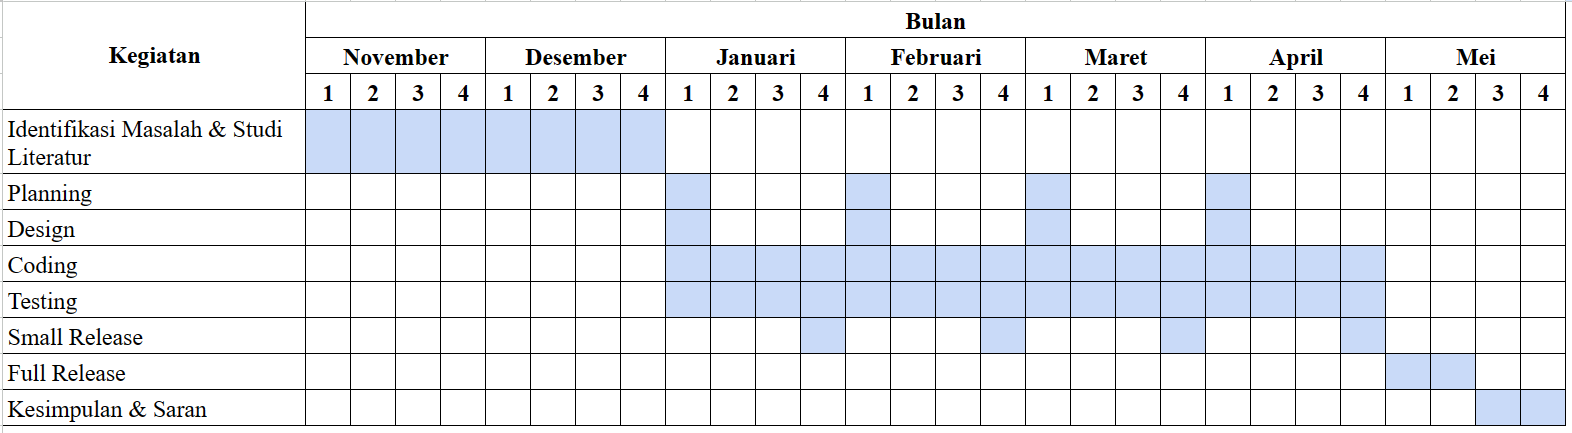
\includegraphics[width=1.2\linewidth, center]{images/metode/schedule.png}
    \caption{Rencana Jadwal Penelitian}
    \label{fig:flow-schedule}
\end{figure}